\documentclass[1p]{elsarticle_modified}
%\bibliographystyle{elsarticle-num}

%\usepackage[colorlinks]{hyperref}
%\usepackage{abbrmath_seonhwa} %\Abb, \Ascr, \Acal ,\Abf, \Afrak
\usepackage{amsfonts}
\usepackage{amssymb}
\usepackage{amsmath}
\usepackage{amsthm}
\usepackage{scalefnt}
\usepackage{amsbsy}
\usepackage{kotex}
\usepackage{caption}
\usepackage{subfig}
\usepackage{color}
\usepackage{graphicx}
\usepackage{xcolor} %% white, black, red, green, blue, cyan, magenta, yellow
\usepackage{float}
\usepackage{setspace}
\usepackage{hyperref}

\usepackage{tikz}
\usetikzlibrary{arrows}

\usepackage{multirow}
\usepackage{array} % fixed length table
\usepackage{hhline}

%%%%%%%%%%%%%%%%%%%%%
\makeatletter
\renewcommand*\env@matrix[1][\arraystretch]{%
	\edef\arraystretch{#1}%
	\hskip -\arraycolsep
	\let\@ifnextchar\new@ifnextchar
	\array{*\c@MaxMatrixCols c}}
\makeatother %https://tex.stackexchange.com/questions/14071/how-can-i-increase-the-line-spacing-in-a-matrix
%%%%%%%%%%%%%%%

\usepackage[normalem]{ulem}

\newcommand{\msout}[1]{\ifmmode\text{\sout{\ensuremath{#1}}}\else\sout{#1}\fi}
%SOURCE: \msout is \stkout macro in https://tex.stackexchange.com/questions/20609/strikeout-in-math-mode

\newcommand{\cancel}[1]{
	\ifmmode
	{\color{red}\msout{#1}}
	\else
	{\color{red}\sout{#1}}
	\fi
}

\newcommand{\add}[1]{
	{\color{blue}\uwave{#1}}
}

\newcommand{\replace}[2]{
	\ifmmode
	{\color{red}\msout{#1}}{\color{blue}\uwave{#2}}
	\else
	{\color{red}\sout{#1}}{\color{blue}\uwave{#2}}
	\fi
}

\newcommand{\Sol}{\mathcal{S}} %segment
\newcommand{\D}{D} %diagram
\newcommand{\A}{\mathcal{A}} %arc


%%%%%%%%%%%%%%%%%%%%%%%%%%%%%5 test

\def\sl{\operatorname{\textup{SL}}(2,\Cbb)}
\def\psl{\operatorname{\textup{PSL}}(2,\Cbb)}
\def\quan{\mkern 1mu \triangleright \mkern 1mu}

\theoremstyle{definition}
\newtheorem{thm}{Theorem}[section]
\newtheorem{prop}[thm]{Proposition}
\newtheorem{lem}[thm]{Lemma}
\newtheorem{ques}[thm]{Question}
\newtheorem{cor}[thm]{Corollary}
\newtheorem{defn}[thm]{Definition}
\newtheorem{exam}[thm]{Example}
\newtheorem{rmk}[thm]{Remark}
\newtheorem{alg}[thm]{Algorithm}

\newcommand{\I}{\sqrt{-1}}
\begin{document}

%\begin{frontmatter}
%
%\title{Boundary parabolic representations of knots up to 8 crossings}
%
%%% Group authors per affiliation:
%\author{Yunhi Cho} 
%\address{Department of Mathematics, University of Seoul, Seoul, Korea}
%\ead{yhcho@uos.ac.kr}
%
%
%\author{Seonhwa Kim} %\fnref{s_kim}}
%\address{Center for Geometry and Physics, Institute for Basic Science, Pohang, 37673, Korea}
%\ead{ryeona17@ibs.re.kr}
%
%\author{Hyuk Kim}
%\address{Department of Mathematical Sciences, Seoul National University, Seoul 08826, Korea}
%\ead{hyukkim@snu.ac.kr}
%
%\author{Seokbeom Yoon}
%\address{Department of Mathematical Sciences, Seoul National University, Seoul, 08826,  Korea}
%\ead{sbyoon15@snu.ac.kr}
%
%\begin{abstract}
%We find all boundary parabolic representation of knots up to 8 crossings.
%
%\end{abstract}
%\begin{keyword}
%    \MSC[2010] 57M25 
%\end{keyword}
%
%\end{frontmatter}

%\linenumbers
%\tableofcontents
%
\newcommand\colored[1]{\textcolor{white}{\rule[-0.35ex]{0.8em}{1.4ex}}\kern-0.8em\color{red} #1}%
%\newcommand\colored[1]{\textcolor{white}{ #1}\kern-2.17ex	\textcolor{white}{ #1}\kern-1.81ex	\textcolor{white}{ #1}\kern-2.15ex\color{red}#1	}

{\Large $\underline{11a_{4}~(K11a_{4})}$}

\setlength{\tabcolsep}{10pt}
\renewcommand{\arraystretch}{1.6}
\vspace{1cm}\begin{tabular}{m{100pt}>{\centering\arraybackslash}m{274pt}}
\multirow{5}{120pt}{
	\centering
	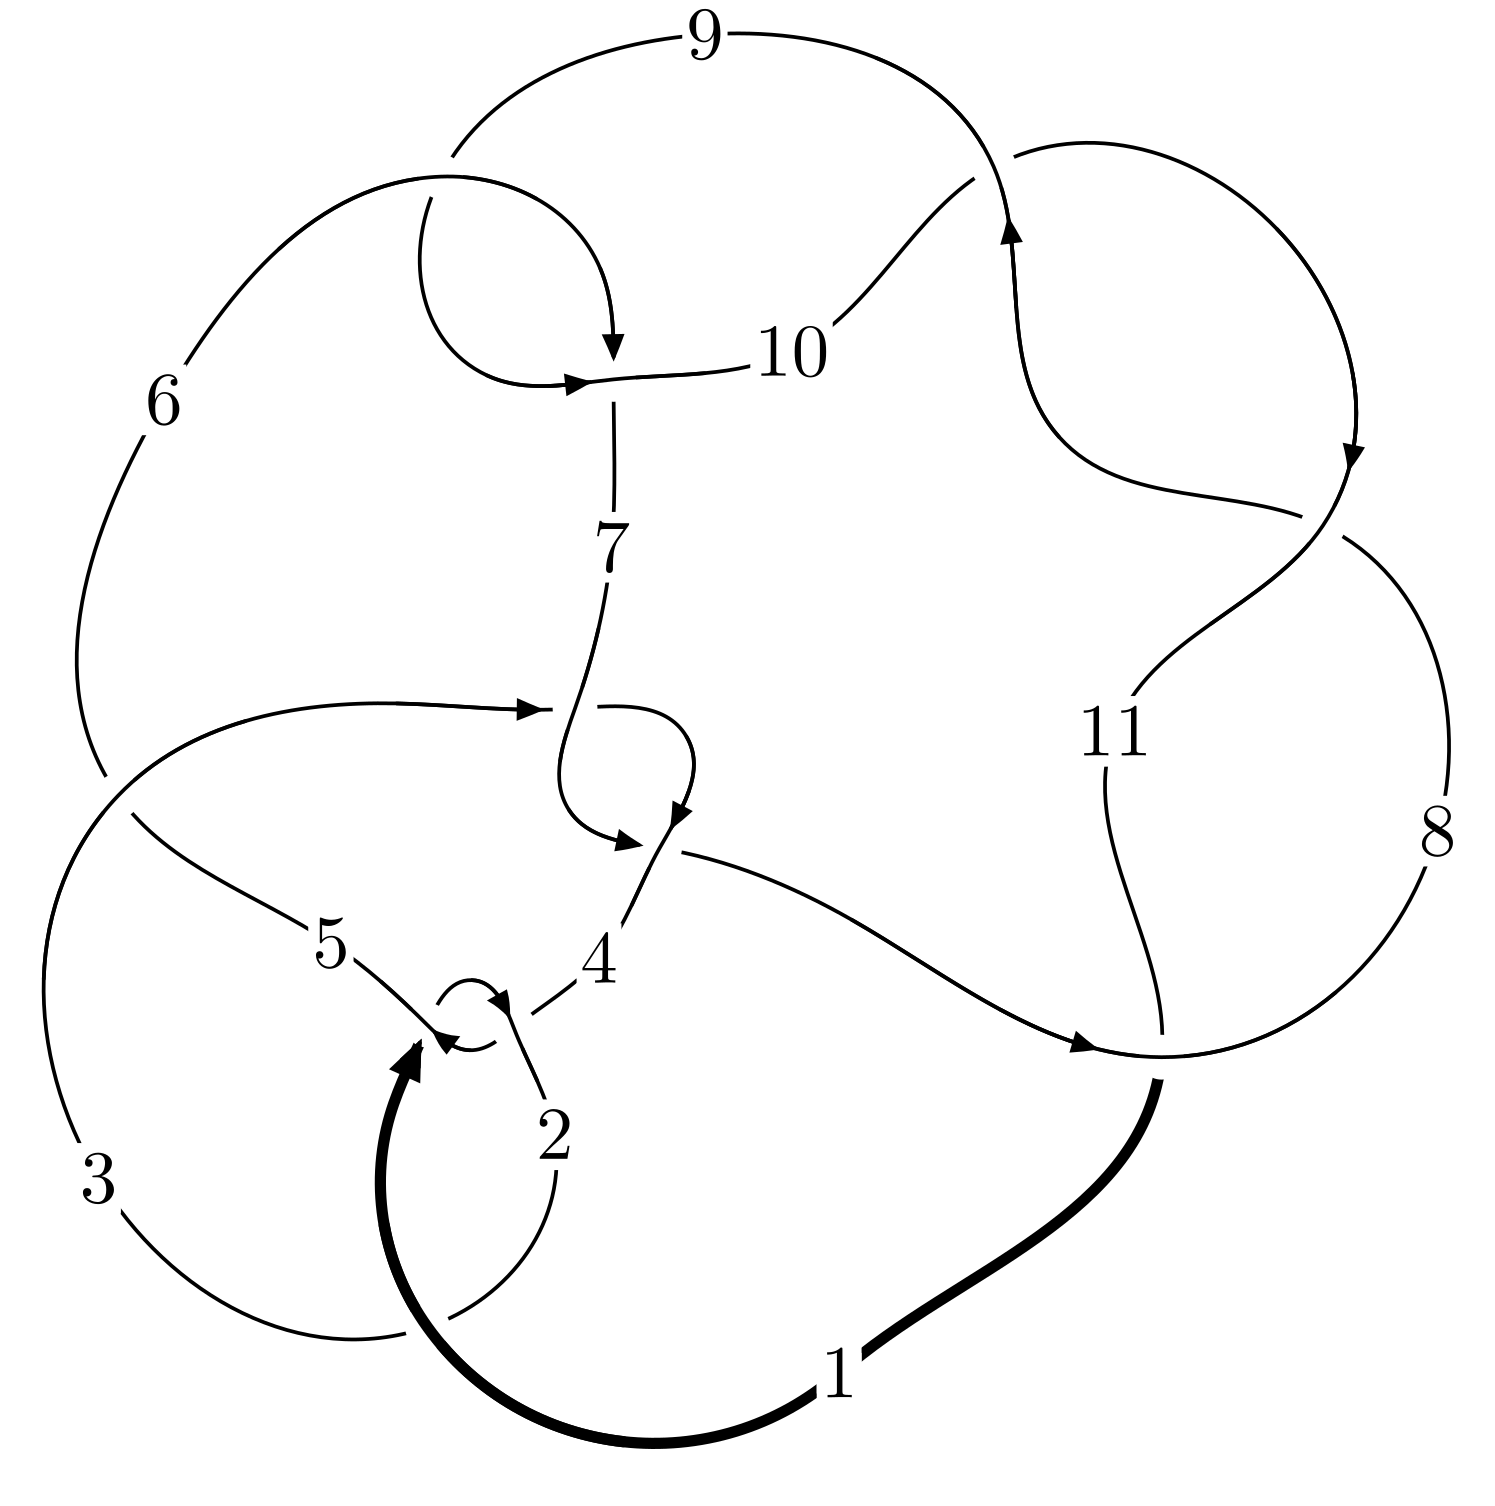
\includegraphics[width=112pt]{../../../GIT/diagram.site/Diagrams/png/253_11a_4.png}\\
\ \ \ A knot diagram\footnotemark}&
\allowdisplaybreaks
\textbf{Linearized knot diagam} \\
\cline{2-2}
 &
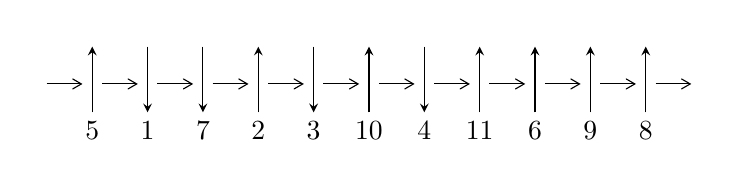
\begin{tikzpicture}[x=20pt, y=17pt]
	% nodes
	\node (C0) at (0, 0) {};
	\node (C1) at (1, 0) {};
	\node (C1U) at (1, +1) {};
	\node (C1D) at (1, -1) {5};

	\node (C2) at (2, 0) {};
	\node (C2U) at (2, +1) {};
	\node (C2D) at (2, -1) {1};

	\node (C3) at (3, 0) {};
	\node (C3U) at (3, +1) {};
	\node (C3D) at (3, -1) {7};

	\node (C4) at (4, 0) {};
	\node (C4U) at (4, +1) {};
	\node (C4D) at (4, -1) {2};

	\node (C5) at (5, 0) {};
	\node (C5U) at (5, +1) {};
	\node (C5D) at (5, -1) {3};

	\node (C6) at (6, 0) {};
	\node (C6U) at (6, +1) {};
	\node (C6D) at (6, -1) {10};

	\node (C7) at (7, 0) {};
	\node (C7U) at (7, +1) {};
	\node (C7D) at (7, -1) {4};

	\node (C8) at (8, 0) {};
	\node (C8U) at (8, +1) {};
	\node (C8D) at (8, -1) {11};

	\node (C9) at (9, 0) {};
	\node (C9U) at (9, +1) {};
	\node (C9D) at (9, -1) {6};

	\node (C10) at (10, 0) {};
	\node (C10U) at (10, +1) {};
	\node (C10D) at (10, -1) {9};

	\node (C11) at (11, 0) {};
	\node (C11U) at (11, +1) {};
	\node (C11D) at (11, -1) {8};
	\node (C12) at (12, 0) {};

	% arrows
	\draw[->,>={angle 60}]
	(C0) edge (C1) (C1) edge (C2) (C2) edge (C3) (C3) edge (C4) (C4) edge (C5) (C5) edge (C6) (C6) edge (C7) (C7) edge (C8) (C8) edge (C9) (C9) edge (C10) (C10) edge (C11) (C11) edge (C12) ;	\draw[->,>=stealth]
	(C1D) edge (C1U) (C2U) edge (C2D) (C3U) edge (C3D) (C4D) edge (C4U) (C5U) edge (C5D) (C6D) edge (C6U) (C7U) edge (C7D) (C8D) edge (C8U) (C9D) edge (C9U) (C10D) edge (C10U) (C11D) edge (C11U) ;
	\end{tikzpicture} \\
\hhline{~~} \\& 
\textbf{Solving Sequence} \\ \cline{2-2} 
 &
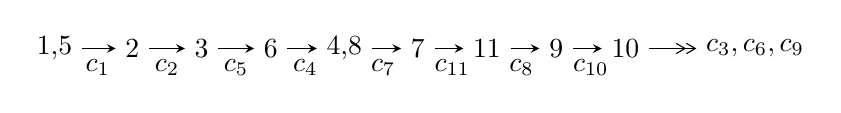
\begin{tikzpicture}[x=25pt, y=7pt]
	% node
	\node (A0) at (-1/8, 0) {1,5};
	\node (A1) at (1, 0) {2};
	\node (A2) at (2, 0) {3};
	\node (A3) at (3, 0) {6};
	\node (A4) at (65/16, 0) {4,8};
	\node (A5) at (41/8, 0) {7};
	\node (A6) at (49/8, 0) {11};
	\node (A7) at (57/8, 0) {9};
	\node (A8) at (65/8, 0) {10};
	\node (C1) at (1/2, -1) {$c_{1}$};
	\node (C2) at (3/2, -1) {$c_{2}$};
	\node (C3) at (5/2, -1) {$c_{5}$};
	\node (C4) at (7/2, -1) {$c_{4}$};
	\node (C5) at (37/8, -1) {$c_{7}$};
	\node (C6) at (45/8, -1) {$c_{11}$};
	\node (C7) at (53/8, -1) {$c_{8}$};
	\node (C8) at (61/8, -1) {$c_{10}$};
	\node (A9) at (10, 0) {$c_{3},c_{6},c_{9}$};

	% edge
	\draw[->,>=stealth]	
	(A0) edge (A1) (A1) edge (A2) (A2) edge (A3) (A3) edge (A4) (A4) edge (A5) (A5) edge (A6) (A6) edge (A7) (A7) edge (A8) ;
	\draw[->>,>={angle 60}]	
	(A8) edge (A9);
\end{tikzpicture} \\ 

\end{tabular} \\

\footnotetext{
The image of knot diagram is generated by the software ``\textbf{Draw programme}" developed by Andrew Bartholomew(\url{http://www.layer8.co.uk/maths/draw/index.htm\#Running-draw}), where we modified some parts for our purpose(\url{https://github.com/CATsTAILs/LinksPainter}).
}\phantom \\ \newline 
\centering \textbf{Ideals for irreducible components\footnotemark of $X_{\text{par}}$} 
 
\begin{align*}
I^u_{1}&=\langle 
-6 u^{53}+25 u^{52}+\cdots+4 b+7,\;7 u^{53}-14 u^{52}+\cdots+4 a+17,\;u^{54}-4 u^{53}+\cdots-5 u+1\rangle \\
I^u_{2}&=\langle 
- a u+b,\;a^3+a^2 u+a^2+2 a u-1,\;u^2+u+1\rangle \\
\\
\end{align*}
\raggedright * 2 irreducible components of $\dim_{\mathbb{C}}=0$, with total 60 representations.\\
\footnotetext{All coefficients of polynomials are rational numbers. But the coefficients are sometimes approximated in decimal forms when there is not enough margin.}
\newpage
\renewcommand{\arraystretch}{1}
\centering \section*{I. $I^u_{1}= \langle -6 u^{53}+25 u^{52}+\cdots+4 b+7,\;7 u^{53}-14 u^{52}+\cdots+4 a+17,\;u^{54}-4 u^{53}+\cdots-5 u+1 \rangle$}
\flushleft \textbf{(i) Arc colorings}\\
\begin{tabular}{m{7pt} m{180pt} m{7pt} m{180pt} }
\flushright $a_{1}=$&$\begin{pmatrix}1\\0\end{pmatrix}$ \\
\flushright $a_{5}=$&$\begin{pmatrix}0\\u\end{pmatrix}$ \\
\flushright $a_{2}=$&$\begin{pmatrix}1\\- u^2\end{pmatrix}$ \\
\flushright $a_{3}=$&$\begin{pmatrix}u^2+1\\- u^2\end{pmatrix}$ \\
\flushright $a_{6}=$&$\begin{pmatrix}- u^5-2 u^3- u\\u^5+u^3+u\end{pmatrix}$ \\
\flushright $a_{4}=$&$\begin{pmatrix}- u\\u^3+u\end{pmatrix}$ \\
\flushright $a_{8}=$&$\begin{pmatrix}-\frac{7}{4} u^{53}+\frac{7}{2} u^{52}+\cdots+\frac{35}{4} u-\frac{17}{4}\\\frac{3}{2} u^{53}-\frac{25}{4} u^{52}+\cdots+12 u-\frac{7}{4}\end{pmatrix}$ \\
\flushright $a_{7}=$&$\begin{pmatrix}-\frac{9}{4} u^{53}+\frac{19}{2} u^{52}+\cdots-\frac{43}{4} u+\frac{1}{4}\\-\frac{1}{2} u^{53}+\frac{9}{4} u^{52}+\cdots+11 u-\frac{9}{4}\end{pmatrix}$ \\
\flushright $a_{11}=$&$\begin{pmatrix}-\frac{1}{4} u^{53}+\frac{3}{4} u^{52}+\cdots+u^2-\frac{5}{4} u\\\frac{1}{4} u^{53}- u^{52}+\cdots+\frac{9}{4} u-\frac{1}{4}\end{pmatrix}$ \\
\flushright $a_{9}=$&$\begin{pmatrix}4 u^{53}-16 u^{52}+\cdots+17 u-\frac{9}{2}\\-\frac{5}{4} u^{53}+\frac{25}{4} u^{52}+\cdots-\frac{39}{4} u+\frac{5}{2}\end{pmatrix}$ \\
\flushright $a_{10}=$&$\begin{pmatrix}\frac{15}{4} u^{53}-\frac{55}{4} u^{52}+\cdots+\frac{41}{4} u-3\\-\frac{5}{4} u^{53}+\frac{29}{4} u^{52}+\cdots-\frac{55}{4} u+\frac{7}{2}\end{pmatrix}$\\ \flushright $a_{10}=$&$\begin{pmatrix}\frac{15}{4} u^{53}-\frac{55}{4} u^{52}+\cdots+\frac{41}{4} u-3\\-\frac{5}{4} u^{53}+\frac{29}{4} u^{52}+\cdots-\frac{55}{4} u+\frac{7}{2}\end{pmatrix}$\\&\end{tabular}
\flushleft \textbf{(ii) Obstruction class $= -1$}\\~\\
\flushleft \textbf{(iii) Cusp Shapes $= -5 u^{53}+\frac{67}{2} u^{52}+\cdots-59 u+16$}\\~\\
\newpage\renewcommand{\arraystretch}{1}
\flushleft \textbf{(iv) u-Polynomials at the component}\newline \\
\begin{tabular}{m{50pt}|m{274pt}}
Crossings & \hspace{64pt}u-Polynomials at each crossing \\
\hline $$\begin{aligned}c_{1},c_{4}\end{aligned}$$&$\begin{aligned}
&u^{54}+4 u^{53}+\cdots+5 u+1
\end{aligned}$\\
\hline $$\begin{aligned}c_{2}\end{aligned}$$&$\begin{aligned}
&u^{54}+28 u^{53}+\cdots+3 u+1
\end{aligned}$\\
\hline $$\begin{aligned}c_{3},c_{7}\end{aligned}$$&$\begin{aligned}
&u^{54}+u^{53}+\cdots+96 u+64
\end{aligned}$\\
\hline $$\begin{aligned}c_{5}\end{aligned}$$&$\begin{aligned}
&u^{54}-4 u^{53}+\cdots-713 u+193
\end{aligned}$\\
\hline $$\begin{aligned}c_{6},c_{9}\end{aligned}$$&$\begin{aligned}
&u^{54}-3 u^{53}+\cdots-2 u+1
\end{aligned}$\\
\hline $$\begin{aligned}c_{8},c_{10},c_{11}\end{aligned}$$&$\begin{aligned}
&u^{54}-13 u^{53}+\cdots+4 u+1
\end{aligned}$\\
\hline
\end{tabular}\\~\\
\newpage\renewcommand{\arraystretch}{1}
\flushleft \textbf{(v) Riley Polynomials at the component}\newline \\
\begin{tabular}{m{50pt}|m{274pt}}
Crossings & \hspace{64pt}Riley Polynomials at each crossing \\
\hline $$\begin{aligned}c_{1},c_{4}\end{aligned}$$&$\begin{aligned}
&y^{54}+28 y^{53}+\cdots+3 y+1
\end{aligned}$\\
\hline $$\begin{aligned}c_{2}\end{aligned}$$&$\begin{aligned}
&y^{54}+56 y^{52}+\cdots+27 y+1
\end{aligned}$\\
\hline $$\begin{aligned}c_{3},c_{7}\end{aligned}$$&$\begin{aligned}
&y^{54}-35 y^{53}+\cdots-54272 y+4096
\end{aligned}$\\
\hline $$\begin{aligned}c_{5}\end{aligned}$$&$\begin{aligned}
&y^{54}-28 y^{53}+\cdots+214995 y+37249
\end{aligned}$\\
\hline $$\begin{aligned}c_{6},c_{9}\end{aligned}$$&$\begin{aligned}
&y^{54}-13 y^{53}+\cdots+4 y+1
\end{aligned}$\\
\hline $$\begin{aligned}c_{8},c_{10},c_{11}\end{aligned}$$&$\begin{aligned}
&y^{54}+59 y^{53}+\cdots-84 y+1
\end{aligned}$\\
\hline
\end{tabular}\\~\\
\newpage\flushleft \textbf{(vi) Complex Volumes and Cusp Shapes}
$$\begin{array}{c|c|c}  
\text{Solutions to }I^u_{1}& \I (\text{vol} + \sqrt{-1}CS) & \text{Cusp shape}\\
 \hline 
\begin{aligned}
u &= -0.379892 + 0.998863 I \\
a &= \phantom{-}1.103900 + 0.557020 I \\
b &= \phantom{-}0.102602 + 0.436031 I\end{aligned}
 & -1.03201 - 1.50079 I & \phantom{-0.000000 } 0 \\ \hline\begin{aligned}
u &= -0.379892 - 0.998863 I \\
a &= \phantom{-}1.103900 - 0.557020 I \\
b &= \phantom{-}0.102602 - 0.436031 I\end{aligned}
 & -1.03201 + 1.50079 I & \phantom{-0.000000 } 0 \\ \hline\begin{aligned}
u &= -0.626212 + 0.684020 I \\
a &= -0.946934 + 0.601830 I \\
b &= \phantom{-}0.572857 - 0.492032 I\end{aligned}
 & \phantom{-}1.52357 - 3.40391 I & \phantom{-}4.82806 + 9.13661 I \\ \hline\begin{aligned}
u &= -0.626212 - 0.684020 I \\
a &= -0.946934 - 0.601830 I \\
b &= \phantom{-}0.572857 + 0.492032 I\end{aligned}
 & \phantom{-}1.52357 + 3.40391 I & \phantom{-}4.82806 - 9.13661 I \\ \hline\begin{aligned}
u &= \phantom{-}0.885029 + 0.254996 I \\
a &= -0.781886 + 1.060890 I \\
b &= \phantom{-}0.24815 - 1.64054 I\end{aligned}
 & -8.53853 - 8.83927 I & -0.16984 + 5.18354 I \\ \hline\begin{aligned}
u &= \phantom{-}0.885029 - 0.254996 I \\
a &= -0.781886 - 1.060890 I \\
b &= \phantom{-}0.24815 + 1.64054 I\end{aligned}
 & -8.53853 + 8.83927 I & -0.16984 - 5.18354 I \\ \hline\begin{aligned}
u &= -0.591212 + 0.904355 I \\
a &= \phantom{-}0.136029 - 0.965536 I \\
b &= \phantom{-}0.452763 + 0.325398 I\end{aligned}
 & \phantom{-}0.88913 - 1.37469 I & \phantom{-0.000000 } 0 \\ \hline\begin{aligned}
u &= -0.591212 - 0.904355 I \\
a &= \phantom{-}0.136029 + 0.965536 I \\
b &= \phantom{-}0.452763 - 0.325398 I\end{aligned}
 & \phantom{-}0.88913 + 1.37469 I & \phantom{-0.000000 } 0 \\ \hline\begin{aligned}
u &= \phantom{-}0.885260 + 0.230562 I \\
a &= \phantom{-}0.737527 - 0.964365 I \\
b &= -0.08283 + 1.52053 I\end{aligned}
 & -8.94569 - 2.41782 I & -0.944300 + 0.387056 I \\ \hline\begin{aligned}
u &= \phantom{-}0.885260 - 0.230562 I \\
a &= \phantom{-}0.737527 + 0.964365 I \\
b &= -0.08283 - 1.52053 I\end{aligned}
 & -8.94569 + 2.41782 I & -0.944300 - 0.387056 I\\
 \hline 
 \end{array}$$\newpage$$\begin{array}{c|c|c}  
\text{Solutions to }I^u_{1}& \I (\text{vol} + \sqrt{-1}CS) & \text{Cusp shape}\\
 \hline 
\begin{aligned}
u &= -0.753157 + 0.805387 I \\
a &= -1.05816 + 1.16882 I \\
b &= \phantom{-}0.15061 - 1.52668 I\end{aligned}
 & -5.15771 - 5.91377 I & \phantom{-0.000000 } 0 \\ \hline\begin{aligned}
u &= -0.753157 - 0.805387 I \\
a &= -1.05816 - 1.16882 I \\
b &= \phantom{-}0.15061 + 1.52668 I\end{aligned}
 & -5.15771 + 5.91377 I & \phantom{-0.000000 } 0 \\ \hline\begin{aligned}
u &= -0.745011 + 0.831417 I \\
a &= \phantom{-}0.96483 - 1.25275 I \\
b &= \phantom{-}0.09191 + 1.50020 I\end{aligned}
 & -5.23505 + 0.31393 I & \phantom{-0.000000 } 0 \\ \hline\begin{aligned}
u &= -0.745011 - 0.831417 I \\
a &= \phantom{-}0.96483 + 1.25275 I \\
b &= \phantom{-}0.09191 - 1.50020 I\end{aligned}
 & -5.23505 - 0.31393 I & \phantom{-0.000000 } 0 \\ \hline\begin{aligned}
u &= -0.499017 + 1.041130 I \\
a &= -0.856626 - 1.113760 I \\
b &= \phantom{-}0.506001 - 0.649056 I\end{aligned}
 & -0.12306 - 4.76592 I & \phantom{-0.000000 } 0 \\ \hline\begin{aligned}
u &= -0.499017 - 1.041130 I \\
a &= -0.856626 + 1.113760 I \\
b &= \phantom{-}0.506001 + 0.649056 I\end{aligned}
 & -0.12306 + 4.76592 I & \phantom{-0.000000 } 0 \\ \hline\begin{aligned}
u &= -0.350126 + 0.758525 I \\
a &= \phantom{-}0.992379 - 0.143031 I \\
b &= -0.0959060 - 0.0489305 I\end{aligned}
 & -0.23114 - 1.44429 I & -1.42255 + 4.98888 I \\ \hline\begin{aligned}
u &= -0.350126 - 0.758525 I \\
a &= \phantom{-}0.992379 + 0.143031 I \\
b &= -0.0959060 + 0.0489305 I\end{aligned}
 & -0.23114 + 1.44429 I & -1.42255 - 4.98888 I \\ \hline\begin{aligned}
u &= \phantom{-}0.188104 + 0.813889 I \\
a &= \phantom{-}1.70541 + 0.20561 I \\
b &= \phantom{-}0.098016 - 1.198770 I\end{aligned}
 & -3.67271 - 1.63897 I & -3.88431 + 4.27010 I \\ \hline\begin{aligned}
u &= \phantom{-}0.188104 - 0.813889 I \\
a &= \phantom{-}1.70541 - 0.20561 I \\
b &= \phantom{-}0.098016 + 1.198770 I\end{aligned}
 & -3.67271 + 1.63897 I & -3.88431 - 4.27010 I\\
 \hline 
 \end{array}$$\newpage$$\begin{array}{c|c|c}  
\text{Solutions to }I^u_{1}& \I (\text{vol} + \sqrt{-1}CS) & \text{Cusp shape}\\
 \hline 
\begin{aligned}
u &= \phantom{-}0.325799 + 1.118780 I \\
a &= \phantom{-}0.231756 + 0.233450 I \\
b &= \phantom{-}0.623088 - 1.028710 I\end{aligned}
 & -4.41304 - 1.91296 I & \phantom{-0.000000 } 0 \\ \hline\begin{aligned}
u &= \phantom{-}0.325799 - 1.118780 I \\
a &= \phantom{-}0.231756 - 0.233450 I \\
b &= \phantom{-}0.623088 + 1.028710 I\end{aligned}
 & -4.41304 + 1.91296 I & \phantom{-0.000000 } 0 \\ \hline\begin{aligned}
u &= \phantom{-}0.461228 + 1.103380 I \\
a &= -0.760887 + 0.869538 I \\
b &= \phantom{-}1.049960 - 0.133110 I\end{aligned}
 & -0.79930 + 3.68471 I & \phantom{-0.000000 } 0 \\ \hline\begin{aligned}
u &= \phantom{-}0.461228 - 1.103380 I \\
a &= -0.760887 - 0.869538 I \\
b &= \phantom{-}1.049960 + 0.133110 I\end{aligned}
 & -0.79930 - 3.68471 I & \phantom{-0.000000 } 0 \\ \hline\begin{aligned}
u &= \phantom{-}0.739810 + 0.258344 I \\
a &= -1.28681 + 0.82591 I \\
b &= \phantom{-}0.734944 - 0.813229 I\end{aligned}
 & -0.37627 - 5.01917 I & \phantom{-}3.74598 + 6.24423 I \\ \hline\begin{aligned}
u &= \phantom{-}0.739810 - 0.258344 I \\
a &= -1.28681 - 0.82591 I \\
b &= \phantom{-}0.734944 + 0.813229 I\end{aligned}
 & -0.37627 + 5.01917 I & \phantom{-}3.74598 - 6.24423 I \\ \hline\begin{aligned}
u &= \phantom{-}0.263878 + 0.734727 I \\
a &= -2.05477 - 0.12446 I \\
b &= \phantom{-}0.313156 + 1.353580 I\end{aligned}
 & -3.33199 + 3.97385 I & -2.23953 - 0.35907 I \\ \hline\begin{aligned}
u &= \phantom{-}0.263878 - 0.734727 I \\
a &= -2.05477 + 0.12446 I \\
b &= \phantom{-}0.313156 - 1.353580 I\end{aligned}
 & -3.33199 - 3.97385 I & -2.23953 + 0.35907 I \\ \hline\begin{aligned}
u &= \phantom{-}0.389551 + 1.166930 I \\
a &= \phantom{-}0.368785 - 0.096490 I \\
b &= -0.342003 + 0.642138 I\end{aligned}
 & -6.05420 + 2.70137 I & \phantom{-0.000000 } 0 \\ \hline\begin{aligned}
u &= \phantom{-}0.389551 - 1.166930 I \\
a &= \phantom{-}0.368785 + 0.096490 I \\
b &= -0.342003 - 0.642138 I\end{aligned}
 & -6.05420 - 2.70137 I & \phantom{-0.000000 } 0\\
 \hline 
 \end{array}$$\newpage$$\begin{array}{c|c|c}  
\text{Solutions to }I^u_{1}& \I (\text{vol} + \sqrt{-1}CS) & \text{Cusp shape}\\
 \hline 
\begin{aligned}
u &= -0.438089 + 1.158700 I \\
a &= \phantom{-}1.57252 + 1.18680 I \\
b &= \phantom{-}0.03942 + 1.53460 I\end{aligned}
 & -7.79249 - 0.92626 I & \phantom{-0.000000 } 0 \\ \hline\begin{aligned}
u &= -0.438089 - 1.158700 I \\
a &= \phantom{-}1.57252 - 1.18680 I \\
b &= \phantom{-}0.03942 - 1.53460 I\end{aligned}
 & -7.79249 + 0.92626 I & \phantom{-0.000000 } 0 \\ \hline\begin{aligned}
u &= -0.459497 + 1.157950 I \\
a &= -1.51732 - 1.29201 I \\
b &= \phantom{-}0.16035 - 1.58211 I\end{aligned}
 & -7.64003 - 7.27340 I & \phantom{-0.000000 } 0 \\ \hline\begin{aligned}
u &= -0.459497 - 1.157950 I \\
a &= -1.51732 + 1.29201 I \\
b &= \phantom{-}0.16035 + 1.58211 I\end{aligned}
 & -7.64003 + 7.27340 I & \phantom{-0.000000 } 0 \\ \hline\begin{aligned}
u &= \phantom{-}0.727484 + 0.127692 I \\
a &= \phantom{-}1.178260 - 0.411070 I \\
b &= -0.306147 + 0.433369 I\end{aligned}
 & -2.35286 - 1.07266 I & -1.50878 + 0.45563 I \\ \hline\begin{aligned}
u &= \phantom{-}0.727484 - 0.127692 I \\
a &= \phantom{-}1.178260 + 0.411070 I \\
b &= -0.306147 - 0.433369 I\end{aligned}
 & -2.35286 + 1.07266 I & -1.50878 - 0.45563 I \\ \hline\begin{aligned}
u &= \phantom{-}0.533177 + 1.145480 I \\
a &= -1.55151 + 0.68284 I \\
b &= \phantom{-}0.838073 + 0.873836 I\end{aligned}
 & -2.97092 + 9.82935 I & \phantom{-0.000000 } 0 \\ \hline\begin{aligned}
u &= \phantom{-}0.533177 - 1.145480 I \\
a &= -1.55151 - 0.68284 I \\
b &= \phantom{-}0.838073 - 0.873836 I\end{aligned}
 & -2.97092 - 9.82935 I & \phantom{-0.000000 } 0 \\ \hline\begin{aligned}
u &= \phantom{-}0.493294 + 1.165470 I \\
a &= \phantom{-}1.239930 - 0.400909 I \\
b &= -0.458261 - 0.419014 I\end{aligned}
 & -5.33044 + 5.62043 I & \phantom{-0.000000 } 0 \\ \hline\begin{aligned}
u &= \phantom{-}0.493294 - 1.165470 I \\
a &= \phantom{-}1.239930 + 0.400909 I \\
b &= -0.458261 + 0.419014 I\end{aligned}
 & -5.33044 - 5.62043 I & \phantom{-0.000000 } 0\\
 \hline 
 \end{array}$$\newpage$$\begin{array}{c|c|c}  
\text{Solutions to }I^u_{1}& \I (\text{vol} + \sqrt{-1}CS) & \text{Cusp shape}\\
 \hline 
\begin{aligned}
u &= \phantom{-}0.272316 + 1.258420 I \\
a &= \phantom{-}0.301237 - 0.770778 I \\
b &= \phantom{-}0.18966 - 1.67412 I\end{aligned}
 & -13.4813 - 5.1046 I & \phantom{-0.000000 } 0 \\ \hline\begin{aligned}
u &= \phantom{-}0.272316 - 1.258420 I \\
a &= \phantom{-}0.301237 + 0.770778 I \\
b &= \phantom{-}0.18966 + 1.67412 I\end{aligned}
 & -13.4813 + 5.1046 I & \phantom{-0.000000 } 0 \\ \hline\begin{aligned}
u &= \phantom{-}0.292425 + 1.259690 I \\
a &= -0.162036 + 0.763414 I \\
b &= -0.05529 + 1.59185 I\end{aligned}
 & -13.77420 + 1.43522 I & \phantom{-0.000000 } 0 \\ \hline\begin{aligned}
u &= \phantom{-}0.292425 - 1.259690 I \\
a &= -0.162036 - 0.763414 I \\
b &= -0.05529 - 1.59185 I\end{aligned}
 & -13.77420 - 1.43522 I & \phantom{-0.000000 } 0 \\ \hline\begin{aligned}
u &= \phantom{-}0.575070 + 1.194170 I \\
a &= -2.04207 + 0.34417 I \\
b &= \phantom{-}0.27962 + 1.66807 I\end{aligned}
 & -11.3710 + 14.1846 I & \phantom{-0.000000 } 0 \\ \hline\begin{aligned}
u &= \phantom{-}0.575070 - 1.194170 I \\
a &= -2.04207 - 0.34417 I \\
b &= \phantom{-}0.27962 - 1.66807 I\end{aligned}
 & -11.3710 - 14.1846 I & \phantom{-0.000000 } 0 \\ \hline\begin{aligned}
u &= \phantom{-}0.564569 + 1.201030 I \\
a &= \phantom{-}1.96539 - 0.25795 I \\
b &= -0.13428 - 1.52301 I\end{aligned}
 & -11.8740 + 7.7158 I & \phantom{-0.000000 } 0 \\ \hline\begin{aligned}
u &= \phantom{-}0.564569 - 1.201030 I \\
a &= \phantom{-}1.96539 + 0.25795 I \\
b &= -0.13428 + 1.52301 I\end{aligned}
 & -11.8740 - 7.7158 I & \phantom{-0.000000 } 0 \\ \hline\begin{aligned}
u &= -0.666189 + 0.031728 I \\
a &= -0.0922958 + 0.0482952 I \\
b &= \phantom{-}0.13196 + 1.49406 I\end{aligned}
 & -4.53071 + 3.08686 I & \phantom{-}1.77023 - 2.56143 I \\ \hline\begin{aligned}
u &= -0.666189 - 0.031728 I \\
a &= -0.0922958 - 0.0482952 I \\
b &= \phantom{-}0.13196 - 1.49406 I\end{aligned}
 & -4.53071 - 3.08686 I & \phantom{-}1.77023 + 2.56143 I\\
 \hline 
 \end{array}$$\newpage$$\begin{array}{c|c|c}  
\text{Solutions to }I^u_{1}& \I (\text{vol} + \sqrt{-1}CS) & \text{Cusp shape}\\
 \hline 
\begin{aligned}
u &= -0.474195 + 0.404040 I \\
a &= -0.896122 + 0.464008 I \\
b &= \phantom{-}0.603365 + 0.428675 I\end{aligned}
 & \phantom{-}1.67487 + 0.64549 I & \phantom{-}7.52215 - 2.21794 I \\ \hline\begin{aligned}
u &= -0.474195 - 0.404040 I \\
a &= -0.896122 - 0.464008 I \\
b &= \phantom{-}0.603365 - 0.428675 I\end{aligned}
 & \phantom{-}1.67487 - 0.64549 I & \phantom{-}7.52215 + 2.21794 I \\ \hline\begin{aligned}
u &= \phantom{-}0.385602 + 0.286567 I \\
a &= -1.99051 + 0.52447 I \\
b &= \phantom{-}0.788212 + 0.173723 I\end{aligned}
 & \phantom{-}1.57101 + 0.14808 I & \phantom{-}6.86906 + 0.36637 I \\ \hline\begin{aligned}
u &= \phantom{-}0.385602 - 0.286567 I \\
a &= -1.99051 - 0.52447 I \\
b &= \phantom{-}0.788212 - 0.173723 I\end{aligned}
 & \phantom{-}1.57101 - 0.14808 I & \phantom{-}6.86906 - 0.36637 I\\
 \hline 
 \end{array}$$\newpage\newpage\renewcommand{\arraystretch}{1}
\centering \section*{II. $I^u_{2}= \langle - a u+b,\;a^3+a^2 u+a^2+2 a u-1,\;u^2+u+1 \rangle$}
\flushleft \textbf{(i) Arc colorings}\\
\begin{tabular}{m{7pt} m{180pt} m{7pt} m{180pt} }
\flushright $a_{1}=$&$\begin{pmatrix}1\\0\end{pmatrix}$ \\
\flushright $a_{5}=$&$\begin{pmatrix}0\\u\end{pmatrix}$ \\
\flushright $a_{2}=$&$\begin{pmatrix}1\\u+1\end{pmatrix}$ \\
\flushright $a_{3}=$&$\begin{pmatrix}- u\\u+1\end{pmatrix}$ \\
\flushright $a_{6}=$&$\begin{pmatrix}-1\\0\end{pmatrix}$ \\
\flushright $a_{4}=$&$\begin{pmatrix}- u\\u+1\end{pmatrix}$ \\
\flushright $a_{8}=$&$\begin{pmatrix}a\\a u\end{pmatrix}$ \\
\flushright $a_{7}=$&$\begin{pmatrix}a\\a u\end{pmatrix}$ \\
\flushright $a_{11}=$&$\begin{pmatrix}a^2 u+1\\- a^2 u- a^2\end{pmatrix}$ \\
\flushright $a_{9}=$&$\begin{pmatrix}a^2 u+a u- a- u-1\\- a^2 u- a^2- a u+1\end{pmatrix}$ \\
\flushright $a_{10}=$&$\begin{pmatrix}- a^2- a- u\\- a^2 u- a^2- a u+1\end{pmatrix}$\\ \flushright $a_{10}=$&$\begin{pmatrix}- a^2- a- u\\- a^2 u- a^2- a u+1\end{pmatrix}$\\&\end{tabular}
\flushleft \textbf{(ii) Obstruction class $= 1$}\\~\\
\flushleft \textbf{(iii) Cusp Shapes $= -3 a^2 u-2 a^2-3 a u+a+7 u+10$}\\~\\
\newpage\renewcommand{\arraystretch}{1}
\flushleft \textbf{(iv) u-Polynomials at the component}\newline \\
\begin{tabular}{m{50pt}|m{274pt}}
Crossings & \hspace{64pt}u-Polynomials at each crossing \\
\hline $$\begin{aligned}c_{1},c_{2},c_{5}\end{aligned}$$&$\begin{aligned}
&(u^2+u+1)^3
\end{aligned}$\\
\hline $$\begin{aligned}c_{3},c_{7}\end{aligned}$$&$\begin{aligned}
&u^6
\end{aligned}$\\
\hline $$\begin{aligned}c_{4}\end{aligned}$$&$\begin{aligned}
&(u^2- u+1)^3
\end{aligned}$\\
\hline $$\begin{aligned}c_{6}\end{aligned}$$&$\begin{aligned}
&(u^3- u^2+1)^2
\end{aligned}$\\
\hline $$\begin{aligned}c_{8}\end{aligned}$$&$\begin{aligned}
&(u^3+u^2+2 u+1)^2
\end{aligned}$\\
\hline $$\begin{aligned}c_{9}\end{aligned}$$&$\begin{aligned}
&(u^3+u^2-1)^2
\end{aligned}$\\
\hline $$\begin{aligned}c_{10},c_{11}\end{aligned}$$&$\begin{aligned}
&(u^3- u^2+2 u-1)^2
\end{aligned}$\\
\hline
\end{tabular}\\~\\
\newpage\renewcommand{\arraystretch}{1}
\flushleft \textbf{(v) Riley Polynomials at the component}\newline \\
\begin{tabular}{m{50pt}|m{274pt}}
Crossings & \hspace{64pt}Riley Polynomials at each crossing \\
\hline $$\begin{aligned}c_{1},c_{2},c_{4}\\c_{5}\end{aligned}$$&$\begin{aligned}
&(y^2+y+1)^3
\end{aligned}$\\
\hline $$\begin{aligned}c_{3},c_{7}\end{aligned}$$&$\begin{aligned}
&y^6
\end{aligned}$\\
\hline $$\begin{aligned}c_{6},c_{9}\end{aligned}$$&$\begin{aligned}
&(y^3- y^2+2 y-1)^2
\end{aligned}$\\
\hline $$\begin{aligned}c_{8},c_{10},c_{11}\end{aligned}$$&$\begin{aligned}
&(y^3+3 y^2+2 y-1)^2
\end{aligned}$\\
\hline
\end{tabular}\\~\\
\newpage\flushleft \textbf{(vi) Complex Volumes and Cusp Shapes}
$$\begin{array}{c|c|c}  
\text{Solutions to }I^u_{2}& \I (\text{vol} + \sqrt{-1}CS) & \text{Cusp shape}\\
 \hline 
\begin{aligned}
u &= -0.500000 + 0.866025 I \\
a &= -1.239560 + 0.467306 I \\
b &= \phantom{-}0.215080 - 1.307140 I\end{aligned}
 & -3.02413 + 0.79824 I & \phantom{-}2.23639 + 1.26697 I \\ \hline\begin{aligned}
u &= -0.500000 + 0.866025 I \\
a &= \phantom{-}1.024480 - 0.839835 I \\
b &= \phantom{-}0.215080 + 1.307140 I\end{aligned}
 & -3.02413 - 4.85801 I & \phantom{-}0.94625 + 7.60556 I \\ \hline\begin{aligned}
u &= -0.500000 + 0.866025 I \\
a &= -0.284920 - 0.493496 I \\
b &= \phantom{-}0.569840\phantom{ +0.000000I}\end{aligned}
 & \phantom{-}1.11345 - 2.02988 I & \phantom{-}5.31735 + 5.84990 I \\ \hline\begin{aligned}
u &= -0.500000 - 0.866025 I \\
a &= \phantom{-}1.024480 + 0.839835 I \\
b &= \phantom{-}0.215080 - 1.307140 I\end{aligned}
 & -3.02413 - 0.79824 I & \phantom{-}2.23639 - 1.26697 I \\ \hline\begin{aligned}
u &= -0.500000 - 0.866025 I \\
a &= -1.239560 - 0.467306 I \\
b &= \phantom{-}0.215080 + 1.307140 I\end{aligned}
 & -3.02413 + 4.85801 I & \phantom{-}0.94625 - 7.60556 I \\ \hline\begin{aligned}
u &= -0.500000 - 0.866025 I \\
a &= -0.284920 + 0.493496 I \\
b &= \phantom{-}0.569840\phantom{ +0.000000I}\end{aligned}
 & \phantom{-}1.11345 + 2.02988 I & \phantom{-}5.31735 - 5.84990 I\\
 \hline 
 \end{array}$$\newpage
\newpage\renewcommand{\arraystretch}{1}
\centering \section*{ III. u-Polynomials}
\begin{tabular}{m{50pt}|m{274pt}}
Crossings & \hspace{64pt}u-Polynomials at each crossing \\
\hline $$\begin{aligned}c_{1}\end{aligned}$$&$\begin{aligned}
&((u^2+u+1)^3)(u^{54}+4 u^{53}+\cdots+5 u+1)
\end{aligned}$\\
\hline $$\begin{aligned}c_{2}\end{aligned}$$&$\begin{aligned}
&((u^2+u+1)^3)(u^{54}+28 u^{53}+\cdots+3 u+1)
\end{aligned}$\\
\hline $$\begin{aligned}c_{3},c_{7}\end{aligned}$$&$\begin{aligned}
&u^6(u^{54}+u^{53}+\cdots+96 u+64)
\end{aligned}$\\
\hline $$\begin{aligned}c_{4}\end{aligned}$$&$\begin{aligned}
&((u^2- u+1)^3)(u^{54}+4 u^{53}+\cdots+5 u+1)
\end{aligned}$\\
\hline $$\begin{aligned}c_{5}\end{aligned}$$&$\begin{aligned}
&((u^2+u+1)^3)(u^{54}-4 u^{53}+\cdots-713 u+193)
\end{aligned}$\\
\hline $$\begin{aligned}c_{6}\end{aligned}$$&$\begin{aligned}
&((u^3- u^2+1)^2)(u^{54}-3 u^{53}+\cdots-2 u+1)
\end{aligned}$\\
\hline $$\begin{aligned}c_{8}\end{aligned}$$&$\begin{aligned}
&((u^3+u^2+2 u+1)^2)(u^{54}-13 u^{53}+\cdots+4 u+1)
\end{aligned}$\\
\hline $$\begin{aligned}c_{9}\end{aligned}$$&$\begin{aligned}
&((u^3+u^2-1)^2)(u^{54}-3 u^{53}+\cdots-2 u+1)
\end{aligned}$\\
\hline $$\begin{aligned}c_{10},c_{11}\end{aligned}$$&$\begin{aligned}
&((u^3- u^2+2 u-1)^2)(u^{54}-13 u^{53}+\cdots+4 u+1)
\end{aligned}$\\
\hline
\end{tabular}\newpage\renewcommand{\arraystretch}{1}
\centering \section*{ IV. Riley Polynomials}
\begin{tabular}{m{50pt}|m{274pt}}
Crossings & \hspace{64pt}Riley Polynomials at each crossing \\
\hline $$\begin{aligned}c_{1},c_{4}\end{aligned}$$&$\begin{aligned}
&((y^2+y+1)^3)(y^{54}+28 y^{53}+\cdots+3 y+1)
\end{aligned}$\\
\hline $$\begin{aligned}c_{2}\end{aligned}$$&$\begin{aligned}
&((y^2+y+1)^3)(y^{54}+56 y^{52}+\cdots+27 y+1)
\end{aligned}$\\
\hline $$\begin{aligned}c_{3},c_{7}\end{aligned}$$&$\begin{aligned}
&y^6(y^{54}-35 y^{53}+\cdots-54272 y+4096)
\end{aligned}$\\
\hline $$\begin{aligned}c_{5}\end{aligned}$$&$\begin{aligned}
&((y^2+y+1)^3)(y^{54}-28 y^{53}+\cdots+214995 y+37249)
\end{aligned}$\\
\hline $$\begin{aligned}c_{6},c_{9}\end{aligned}$$&$\begin{aligned}
&((y^3- y^2+2 y-1)^2)(y^{54}-13 y^{53}+\cdots+4 y+1)
\end{aligned}$\\
\hline $$\begin{aligned}c_{8},c_{10},c_{11}\end{aligned}$$&$\begin{aligned}
&((y^3+3 y^2+2 y-1)^2)(y^{54}+59 y^{53}+\cdots-84 y+1)
\end{aligned}$\\
\hline
\end{tabular}
\vskip 2pc
\end{document}